\documentclass{article}
\usepackage{graphicx}
\usepackage{amssymb}
\usepackage{geometry}
\usepackage{bm}
\usepackage{fancyhdr}
\usepackage{minted}
\usepackage{amsmath}
\pagestyle{plain}
\title{CMSE890 Project Report}
\author{Haiyang Yu}
\date{}
\begin{document}
\maketitle

\subsection*{1.Background and Question}
In statistics, parameters estimation is an important component. Maximum Likelihood Estimation (MLE) is the method to estimate parameters by maximizing the likelihood function. Suppose the parameter is $\theta$ in parameter space $\Theta$. The observed sample $\bm{y}=\{y_{1},y_{2},\cdots y_{n}\}$ has the distribution $f(\bm{y},\theta)$ where parameters $\theta$ is unknown. To get the best estimation $\hat{\theta}$, MLE maximize the likelihood function 
$$\hat{\theta}=\mathop{\arg\max}_{\theta\in\Theta}f(\bm{y},\theta)$$
In general, we take the derivatives for the log-likelihood function and let it be 0 to get the analytical solution of $\hat{\theta}$.
$$\frac{\partial \log{f(\bm{y},\theta)}}{\partial \theta}=0$$
However, some likelihood functions have latent variable $z$ that we cannot get the closed form solution. In this case, many people use EM algorithm to get the numerical solution of $\hat{\theta}$. EM algorithm has 2 steps to get the maximum. The first step is using the initial parameter $\theta_{0}$ to calculate the $Q$ function.
The second step is to maximize the $Q$ function. And enter the next iteration. It has been proved that EM algorithm converges. But if we regard it as an optimization problem, can we apply the optimization methods on the likelihood function, and is it more efficient than EM?
\subsection*{2.EM Algorithm}
\subsubsection*{E Step(Expactation Step)}

$$Q(\theta|\theta^{(t)})=\mathrm{E}_{z|\bm{y}}(\log{L(\bm{y},z,\theta)})$$as the conditional expactation given $x$ and $\theta$.

\subsubsection*{M Step(Maximum Step)}
$$\theta^{(t+1)}=\mathop{\arg\max}_{\theta}Q(\theta|\theta^{(t)})$$
\subsection*{3.Model} 
 You have 3 coins $A,B$ and $C$. First, you toss coin $A$. If it is positive side, you toss coin $B$, else you toss coin $C$, and write down the side types. What has been observed is the side of coin $B$ and $C$ like "$0,1,1,0,1,\cdots$". We don't know whether the result is from coin $B$ or coin $C$. Suppose the positive-side probability of coins $A,B,C$ is $\pi,p,q$, then use the observed data to estimate $\pi,p,q$.

\subsection*{4.Analysis}
In this model, the Maximum likelihood function is
$$L(\bm{y},\theta)=\prod_{i=1}^{n}(\pi p^{y_{i}}(1-p)^{1-y_{i}}+(1-\pi)q^{y_{i}}(1-q)^{1-y_{i}})$$
We introduce the latent variable $z$, which means the result from coin $B$ or coin $C$.
The likelihood function becomes $$L(\bm{y},z,\theta)=\sum_{z}P(z|\theta)P(\bm{y}|z,\theta)$$

\subsection*{5.Results}
For the model of three coins, it doesn't have a closed form. But in the EM algorithm, M step has the closed form. We choose 4 methods(SGD,GD,EM with GD optimizer,EM with closed form) to compare their iterations and speed.

\begin{center}
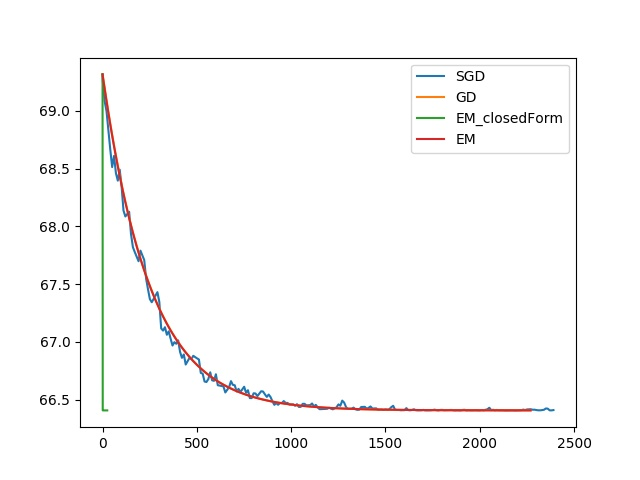
\includegraphics[width=10cm]{sgd.jpg} 
\end{center}


\begin{center}
\begin{tabular}{|c|c|}
\hline
Method & Time\\
\hline
SGD     &         0.65s\\
\hline
GD        &        1.34s\\
\hline
EM(closedForm)     &        0.06s\\
\hline
EM(GD)          &    7.32s\\
\hline
\end{tabular}
\end{center}

\subsection*{6.Conclusion}

\noindent 1. If the optimization doesn't has the closed form and M-step has the closed form, EM algorithm converges much faster than the same optimization method.

\noindent 2. If not, EM is slower with the same optimization method.

\noindent 3. EM algorithm is very helpful in some model like Gaussian mix model, which has closed form in EM algorithm but not in regular optimization method.

\subsection*{Appendix}
\begin{minted}{python}
import numpy as np
import matplotlib.pyplot as plt
import random
import time

np.random.seed(1234)
###real para  pi=0.4  p=0.5  q=0.8
###if head 1, else 0
###fOpt=66.40641266
fOpt=66.40641266
y=[1, 1, 1, 0, 1, 0, 1, 1, 1, 1, 0, 1, 1, 1, 0, 1, 1, 0, 1, 0, 1, 1, 1, 1,
   1, 1, 0, 1, 0, 0, 1, 0, 1, 1, 0, 0, 1, 0, 1, 1, 1, 1, 0, 1, 0, 1, 1, 1,
   0, 1, 0, 1, 1, 1, 1, 1, 1, 0, 0, 0, 0, 1, 1, 1, 0, 1, 1, 1, 0, 0, 1, 1,
   1, 0, 1, 0, 1, 0, 1, 0, 1, 0, 0, 1, 1, 0, 1, 0, 0, 1, 0, 1, 0, 1, 1, 0, 1, 1, 0, 0]
eps=1e-6
def generateSample(n):
    res=[]
    for _ in range(n):
        coin=1
        i=random.random()
        if i>0.4:
            coin=2
        if coin==1:
            j=random.random()
            if j>0.5:
                r=1
            else:
                r=0
        else:
            j=random.random()
            if j>0.7:
                r=0
            else:
                r=1
        res.append(r)
    return res

def f(y,pi,p,q):
    if y==1:
        res=pi*p+(1-pi)*q
    else:
        res=pi*(1-p)+(1-pi)*(1-q)
    return -np.log(res)

def F(pi,p,q):
    sm=0
    for i in range(len(y)):
        sm+=f(y[i],pi,p,q)
    return sm

def dfdpi(y,pi,p,q):
    if y==1:
        res=(q-p)/(pi*p+(1-pi)*q)
    else:
        res=(p-q)/(pi*(1-p)+(1-pi)*(1-q))
    return res

def dfdp(y,pi,p,q):
    if y==1:
        res=-pi/(pi*p+(1-pi)*q)
    else:
        res=pi/(pi*(1-p)+(1-pi)*(1-q))
    return res

def dfdq(y,pi,p,q):
    if y==1:
        res=(pi-1)/(pi*p+(1-pi)*q)
    else:
        res=(1-pi)/(pi*(1-p)+(1-pi)*(1-q))
    return res

def sgd():
    ##init pi=1,p=1,q=0.5
    n=len(y)
    alpha=0.00001
    iter=1
    yarr=[]
    pi=0.5
    p=0.5
    q=0.5
    yarr.append(F(pi,p,q))
    k=0
    x=[0]
    while iter<25:
        pre=F(pi,p,q)
        flag=0
        index = random.sample(range(n), n)
        for j in range(len(index)):
            pi = pi - alpha *n* dfdpi(y[index[j]], pi, p, q)
            p = p - alpha *n* dfdp(y[index[j]], pi, p, q)
            q = q - alpha *n* dfdq(y[index[j]], pi, p, q)
            k+=1
            val = F(pi, p, q)
            if abs(val - pre) < eps:
                flag = 1
                break
            if j%10==0:
                yarr.append(val)
                x.append(k)
        if flag==1:
                break
        iter+=1
    print(k)
    plt.plot(x,yarr,label='SGD')

def gd():
    ##init pi=1,p=1,q=0.5
    n = len(y)
    alpha = 0.00001
    yarr = []
    pi = 0.5
    p = 0.5
    q = 0.5
    yarr.append(F(pi, p, q))
    k = 0
    x = [0]
    while k < 2500:
        val = F(pi, p, q)
        dpi=0
        dp=0
        dq=0
        for i in range(n):
            dpi+=dfdpi(y[i],pi,p,q)
            dp+=dfdp(y[i],pi,p,q)
            dq+=dfdq(y[i],pi,p,q)
        pi = pi - alpha * dpi
        p = p - alpha * dp
        q = q - alpha * dq
        k += 1
        if abs(val-F(pi,p,q))<eps:
            break
        if k % 10 == 0:
            yarr.append(val)
            x.append(k)
    print(k)
    plt.plot(x, yarr,label='GD')


def em():
    n = len(y)
    alpha = 0.00001
    yarr = []
    pi = 0.5
    p = 0.5
    q = 0.5
    yarr.append(F(pi, p, q))
    k = 0
    x = [0]
    mu=np.zeros((n,1))
    while k<25:
        for i in range(n):
            if y[i]==1:
                mu[i]=pi*p/(pi*p+(1-pi)*q)
            else:
                mu[i]=pi*(1-p)/(pi*(1-p)+(1-pi)*(1-q))
        sm=sum(mu)
        pi=sm/n
        r1=0
        r2=0
        for i in range(n):
            r1+=mu[i]*y[i]
            r2+=(1-mu[i])*y[i]
        p=r1/sm
        q=r2/(n-sm)
        k+=1
        if k % 1 == 0:
            yarr.append(F(pi,p,q))
            x.append(k)
    plt.plot(x, yarr, label='EM_closedForm')

def Q(mu,y,pi,p,q):
    n=len(mu)
    res=0
    for i in range(n):
        tmp=mu[i]*np.log(pi*p**y[i]*(1-p)**(1-y[i]))+(1-mu[i])*np.log((1-pi)*q**y[i]*(1-q)**(1-y[i]))
        res+=tmp
    return -res
def dQdpi(mu,y,pi,p,q):
    n = len(mu)
    res = 0
    for i in range(n):
        tmp=(mu[i]-pi)/(pi*(1-pi))
        res+=tmp
    return -res

def dQdp(mu,y,pi,p,q):
    n = len(mu)
    res = 0
    for i in range(n):
        tmp=mu[i]*(y[i]-p)/(p*(1-p))
        res+=tmp
    return -res
def dQdq(mu,y,pi,p,q):
    n = len(mu)
    res = 0
    for i in range(n):
        tmp=(1-mu[i])*(y[i]-q)/(q*(1-q))
        res+=tmp
    return -res

def emIter():
    n = len(y)
    alpha = 0.00001
    yarr = []
    pi = 0.5
    p = 0.5
    q = 0.5
    yarr.append(F(pi, p, q))
    k = 0
    x = [0]
    mu=np.zeros((n,1))
    while k<2500:
        flag=0
        for i in range(n):
            if y[i]==1:
                mu[i]=pi*p/(pi*p+(1-pi)*q)
            else:
                mu[i]=pi*(1-p)/(pi*(1-p)+(1-pi)*(1-q))
        for iter in range(100):
            val=F(pi,p,q)
            pi=pi-alpha*dQdpi(mu,y,pi,p,q)
            p = p - alpha * dQdp(mu, y, pi, p, q)
            q = q - alpha * dQdq(mu, y, pi, p, q)
            k += 1
            if abs(F(pi,p,q)-val)<eps:
                flag=1
                break
            if k%10==0:
                yarr.append(F(pi,p,q))
                x.append(k)
        if flag == 1:
            break
    print(k)
    plt.plot(x, yarr,label='EM')

if __name__=="__main__":
    begin=time.clock()
    sgd()
    gd()
    em()
    emIter()
    end=time.clock()
    plt.legend()
    plt.savefig("sgd.jpg")
    plt.show()
    '''
    begin1=time.clock()
    gd()
    end1=time.clock()
    begin2=time.clock()
    emIter()
    end2=time.clock()
    plt.legend()
    plt.show()
    print(end-begin,end1-begin1,end2-begin2)
    '''


\end{minted}

\end{document}